\chapter{Experimentos}
\label{cap:experiments}

\section{Ambiente de simulação}

Uma simulação da rede nacional de pesquisa, a rede Ipê \citep{ipe2015network} 
foi criada em laboratório.
Um comutador (\emph{switch}) OpenFlow e quatro servidores foram utilizados 
para executar a simulação no laboratório WiNet \citep{winet22015lab}
no departamento de Ciência da Computação (DCC) da Universidade Federal 
de Minas Gerais (UFMG).

\subsection{A rede Ipê}
Operada pela Rede Nacioanal de Pesquisa (RNP), a rede Ipê é uma infraestrutura
de rede Internet dedicada à comunidade de pesquisa brasileira.
Inaugurada em 2005, foi a primeira rede óptica nacional acadêmica a entrar em
operação na América Latina.

A rede IPÊ implementa 27 Pontos de Presença (\emph{POPs}), um para cada unidade
da federação.
Em cada unidade existem diversos clientes que, para se comunicar com outras 
máquinas em outros Pontos de Presença, transmitem seus pacotes através do 
POP ao qual atuam como clientes.
Essas ramificações constituem mais de 800 instituições de ensino, saúde e 
pesquisa em todo o país, beneficiando mais de 3,5 milhões de usuários
\citep{ipe2015network}.

Através da rede RedCLARA \citep{redclara2015network}, a rede Ipê se conecta 
à 2,5 Gb/s com, atualmente, 15 países da América Latina e à 5 Gb/s com a rede
europeia Géant \citep{geant2015network}. 
Além disso, por meio de quatro conexões de
10 Gb/s, duas pelo Oceano Atlântico e duas pelo Oceano Pacífico, 
operadas em parceria com a ANSP, totalizando 40 Gb/s, a rede Ipê se conecta 
às redes acadêmicas norte-americanas, em especial, a  Internet2 
\citep{internet22015network}, a outras redes acadêmicas internacionais e à 
internet comercial mundial.

Os Pontos de presença estão interconectados conforme mostrado na figura 
\ref{fig:ipe-network-2015}.

\begin{figure}[!ht]
    \centering
    \label{fig:ipe-network-2015}
    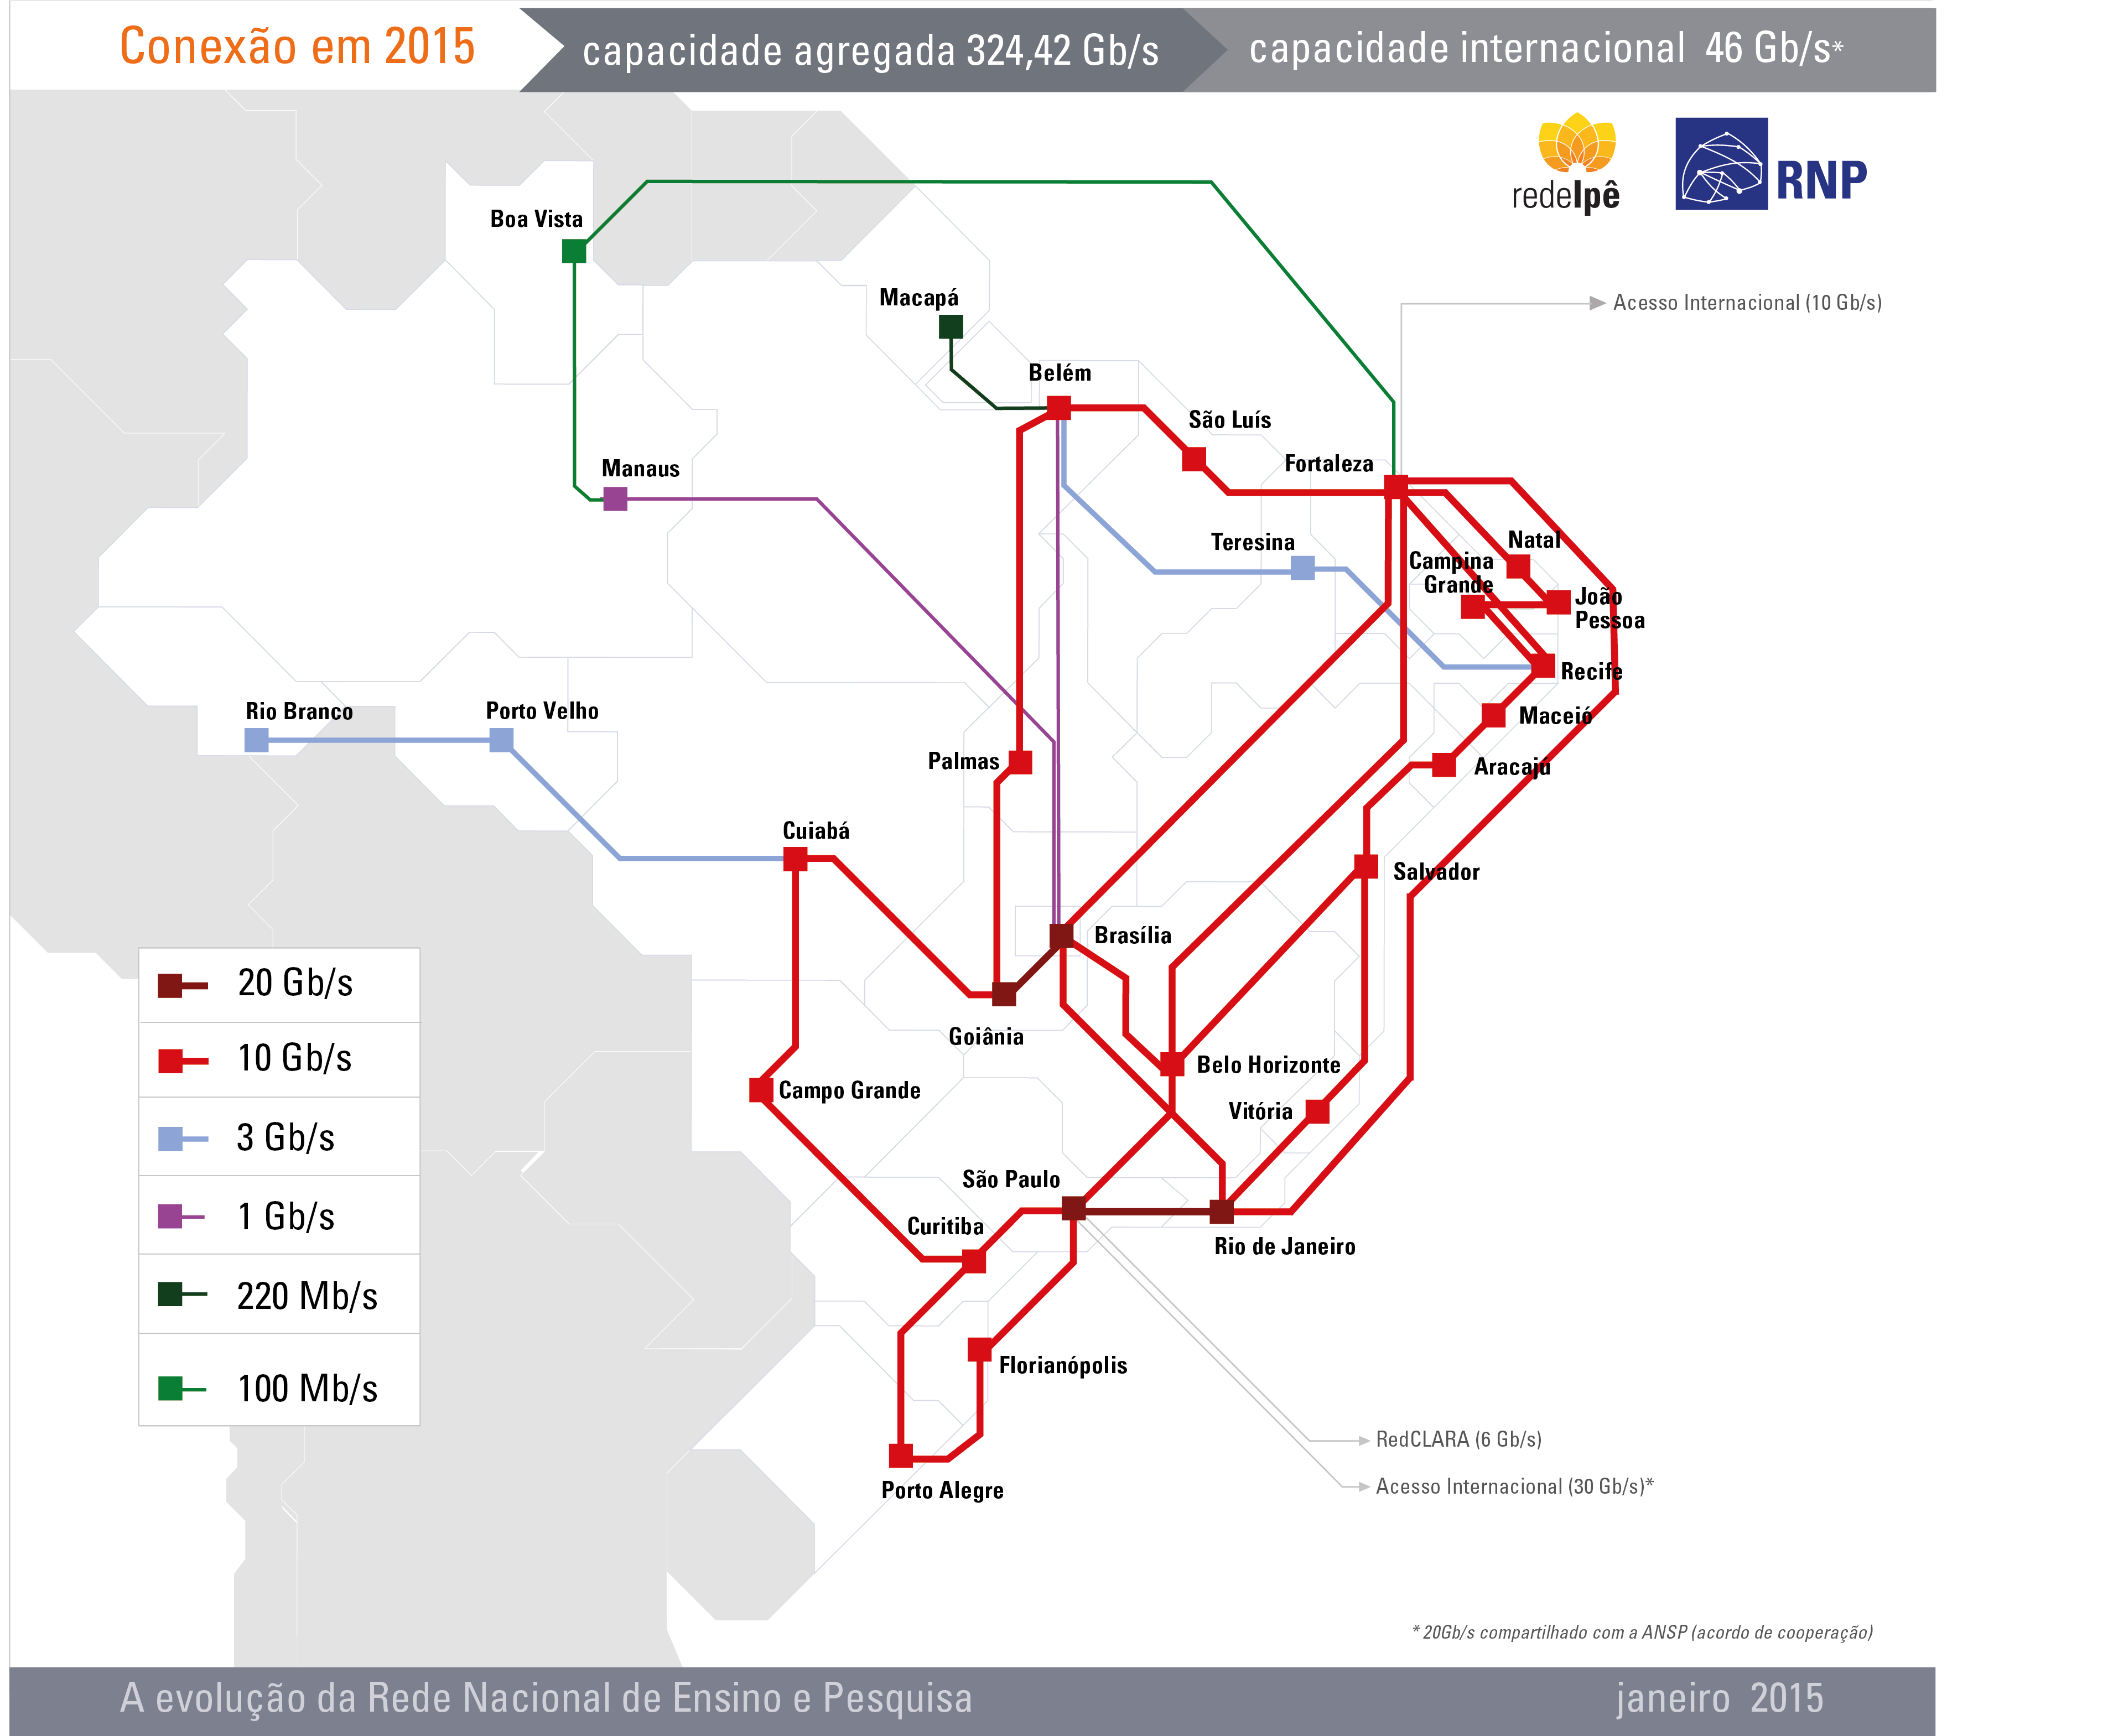
\includegraphics[width=\textwidth]{img/ipe-network-2015}
    \caption{Rede Nacional de Pesquisa IPÊ \protect\footnotemark}
    \vspace*{3in}
\end{figure}

\footnotetext{Imagem retirada de 
\url{http://www.rnp.br/servicos/conectividade/rede-ipe}}

\subsection{Arquitetura da simulação}

A ambiente de simulação é composto por um comutador HP com OpenFlow habilitado.
Quatro servidores são responsáveis por gerenciar máquinas virtuais que 
representam as unidades federativas e suas instituições clientes.

Conforme pode ser visto na figura \ref{fig:physical-vs-virtual-network}, a
rede física do esperimento é separada da rede virtual.
O quinto computador é o controlador da rede. 
Para o experimento, existem duas redes. 
Uma rede de administração, com acesso aos servidores e a uma instância do 
controlador, na porta 6633.
A segunda rede é a rede virtual à qual todos os POPs simulados estão 
conectados. 
Para implementar essas duas redes, cada servidor e o controlador possuem duas
interfaces de rede que isolam seus funcionamentos.
Assim, a rede física/administrativa e a rede virtual/Ipê estão separadas
em nosso experimento.


\begin{figure}[!h]
    \centering
    \label{fig:physical-vs-virtual-network}
    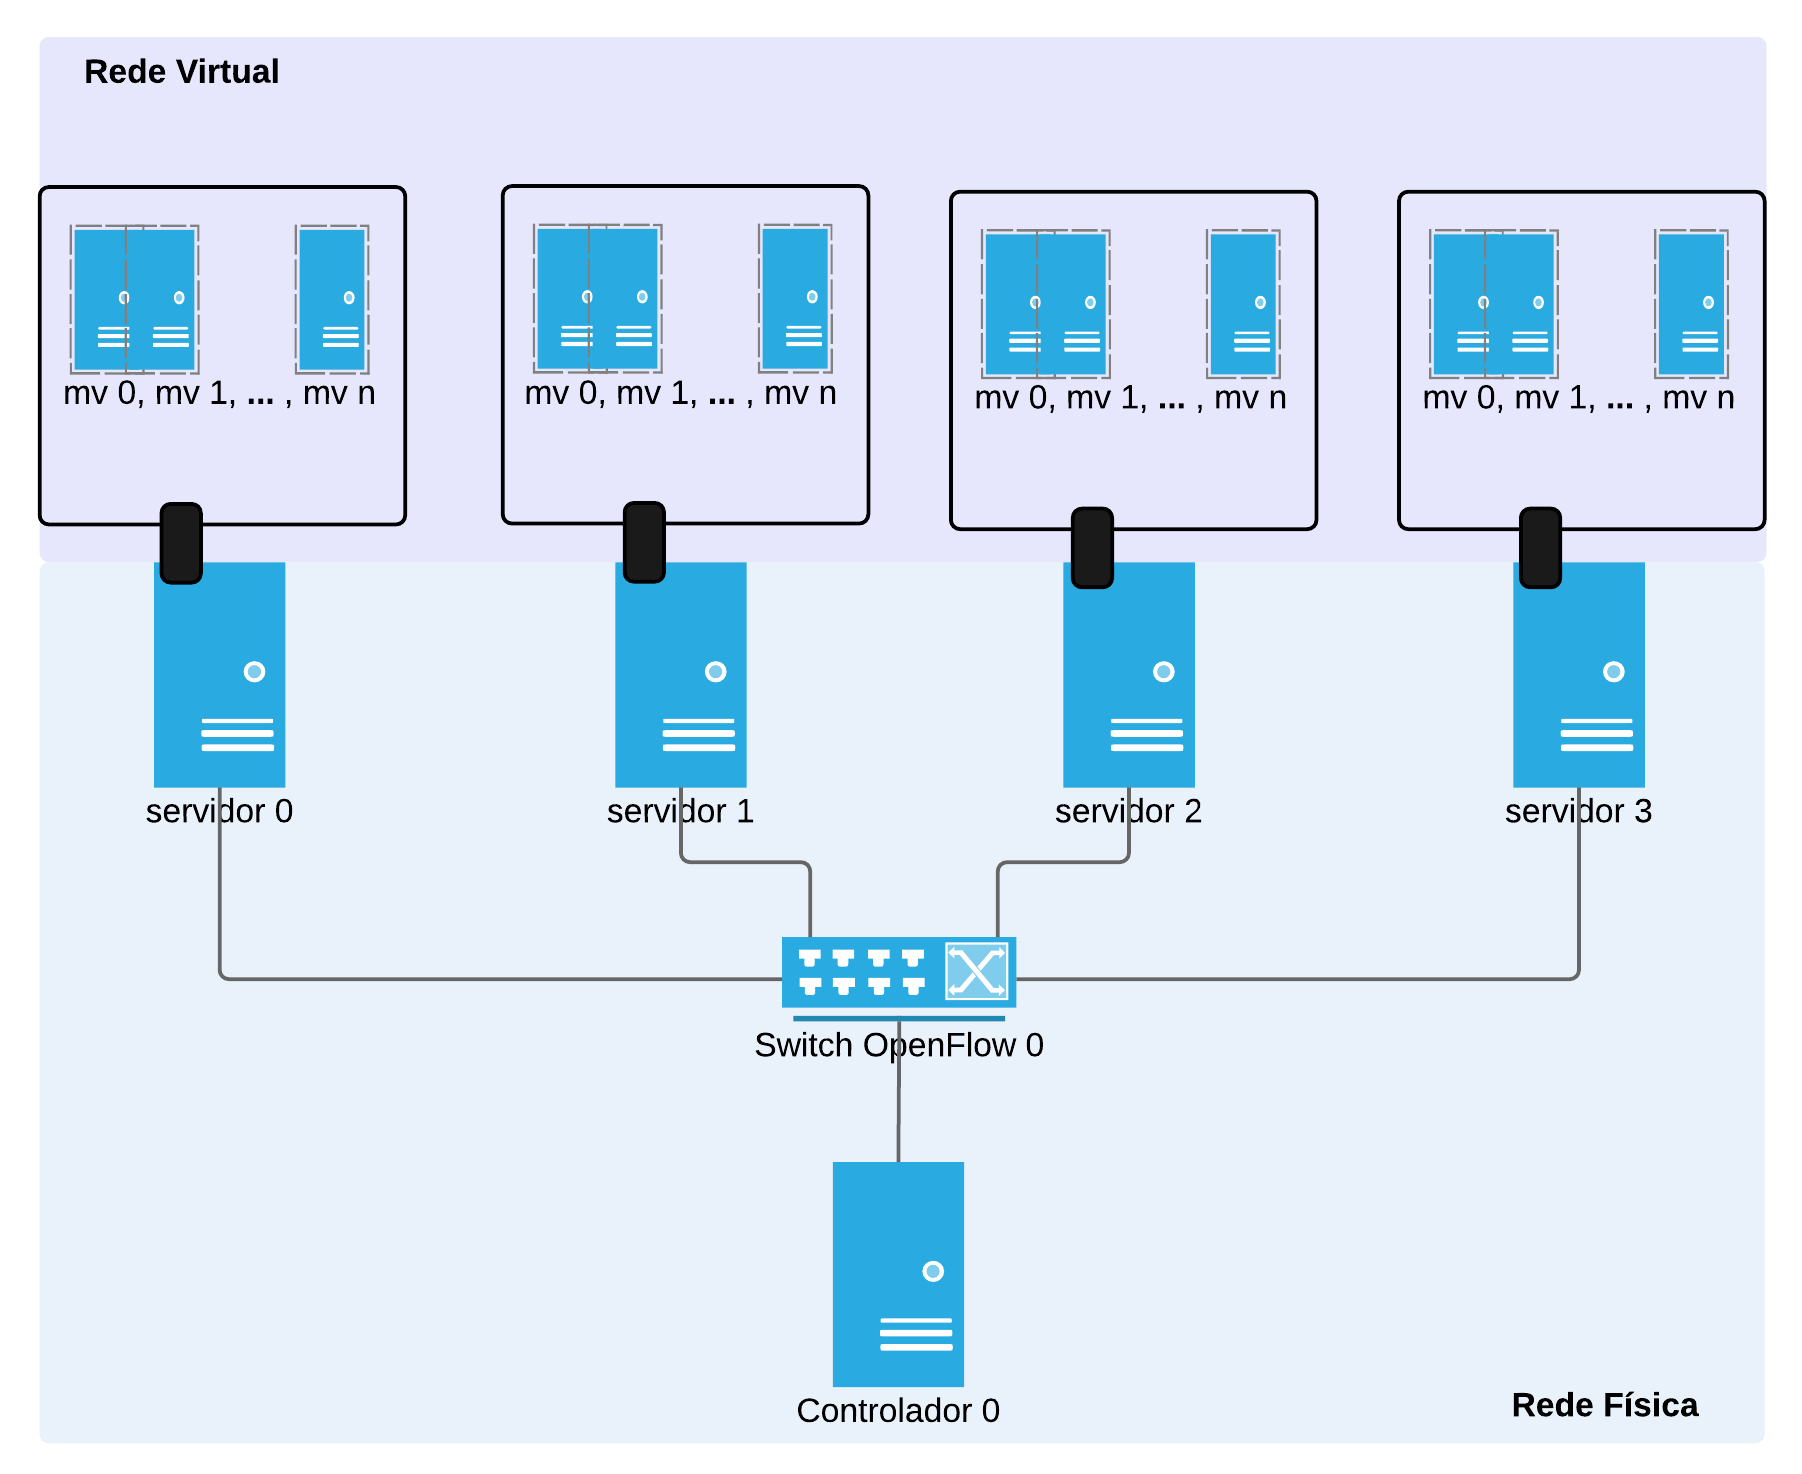
\includegraphics[width=\textwidth]{img/physical-vs-virtual-network-pt}
    \caption{Arquitetura do ambiente de simulação}
\end{figure}

Para o ambiente virtualizado, o controlador está associado a porta 6653.
Cada POP é um comutador (\emph{switch}) OpenFlow simulado via OpenVSwitch
\citep{openvswitch2015switch}.
As instituições clientes de cada POP são simuladas através do \emph{Mininet} 
\citep{lantz2010network}.
O número de instituições clientes foi coletado do sítio de cada Ponto de 
Presença.

Cada máquina virtual representa um POP.
Cada POP possui uma subrede à qual uma instância do \emph{Mininet} simula 
seus clientes. 
Essa subrede está conectada através de um \emph{switch} virtual 
\emph{OpenVSwitch} que é controlado pelo controlador da rede virtualizada.
Assim, para cada POP, temos as decisões e atualizações da tabela de fluxos
feita pelo controlador.
A tabela \ref{tbl:testbed-ipe-net} apresenta as subredes de cada unidade
federativa (POP), qual servidor físico gerencia a máquina virtual referente
ao POP e o número de clientes a ele associado.

\begin{table}[h]
    \label{tbl:testbed-ipe-net}
    \centering
    \resizebox*{!}{\dimexpr\textheight- 25px}{
    \resizebox{\linewidth}{!}{
    \begin{tabular}{llllll}
        \rowcolor[HTML]{000000} 
        \multicolumn{6}{c}{\cellcolor[HTML]{000000}{\color[HTML]{C0C0C0} 
            \textbf{Associação de Servidores à simulação da rede IPÊ}}} \\
        \rowcolor[HTML]{000000} 
        {\color[HTML]{9B9B9B} \textbf{UF}} & {\color[HTML]{9B9B9B} 
            \textbf{N clientes}} & {\color[HTML]{9B9B9B} 
            \textbf{Sub-rede local}} & {\color[HTML]{9B9B9B} 
            \textbf{Servidor}} & {\color[HTML]{9B9B9B} \textbf{IP local}} & 
            {\color[HTML]{9B9B9B} \textbf{IP Gateway}} \\
        AC &  10 &  10.10.1.0 &   Shiva  &  10.10.42.51 & \\ 
        AL  & 13 &  10.10.2.0  &  Shiva  &  10.10.42.52 & \\ 
        AM  & 20 &  10.10.3.0 &   Shiva  &  10.10.42.53 & \\
        AP  & 7  &  10.10.4.0 &   Shiva  &  10.10.42.54 & 10.10.42.50 \\
        BA  & 25 &  10.10.5.0 &   Shiva  &  10.10.42.55 & \\
        CE  & 50  & 10.10.6.0  &  Shiva  &  10.10.42.56 & \\
        DF  & 16 &  10.10.7.0  &  Shiva  &  10.10.42.57 & \\ \hline
        ES  & 26  & 10.10.8.0  &  Eden  &   10.10.42.101 & \\
        GO  & 26  & 10.10.9.0  &  Eden  &   10.10.42.102  & \\  
        MA  & 7  &  10.10.10.0 &  Eden  &   10.10.42.103  & \\  
        MG  & 32  & 10.10.11.0  & Eden  &   10.10.42.104  & 10.10.42.100 \\  
        MS  & 10  & 10.10.12.0  & Eden  &   10.10.42.105  & \\  
        MT  & 8   & 10.10.13.0  & Eden  &   10.10.42.106  & \\  
        PA  & 13  & 10.10.14.0  & Eden  &   10.10.42.107  & \\ \hline
        PB  & 14  & 10.10.15.0  & Diablos & 10.10.42.151  & \\
        PE  & 41  & 10.10.16.0  & Diablos & 10.10.42.152  & \\  
        PI &  25 &  10.10.17.0 &  Diablos & 10.10.42.153  & \\  
        PR &  71 &  10.10.18.0 &  Diablos & 10.10.42.154  & 10.10.42.150 \\
        RJ &  27 &  10.10.19.0 &  Diablos & 10.10.42.155  & \\  
        RN &  11 &  10.10.20.0 &  Diablos & 10.10.42.156  & \\  
        RO &  10 &  10.10.21.0 &  Diablos & 10.10.42.157  & \\ \hline
        RR  & 7  &  10.10.22.0 &  Leviathan &   10.10.42.201 & \\
        RS &  10 &  10.10.23.0 &  Leviathan &   10.10.42.202  & \\  
        SC &  47 &  10.10.24.0 &  Leviathan &   10.10.42.203 & 10.10.42.200 \\   
        SE &  13 &  10.10.25.0 &  Leviathan &   10.10.42.204 & \\   
        SP &  25 &  10.10.26.0 &  Leviathan &   10.10.42.205  & \\  
        TO &  11 &  10.10.27.0 &  Leviathan &   10.10.42.206 & \\   
    \end{tabular}
    }}
\end{table}


\section{Detecção de entidades}

Ao ser carregado, o módulo \emph{graph} inicia o grafo da rede vazio.
Os \emph{switches} são os primeiros a serem identificados. 
Como o controlador está ligado diretamente a eles pela interface
\emph{OpenFlow}, um evento de \emph{ConnectionUp} é disparado 
pelo núcleo do controlador.
Esse evento dispara o evento \emph{SwitchJoin} através do módulo 
\emph{topology} que faz com que o grafo adicione vértices.

\begin{figure}[h!]
    \centering
    \begin{lstlisting}[ tabsize=4,  
                        language=bash,
                        basicstyle=\ttfamily\footnotesize,
                        aboveskip={1.5\baselineskip},
                        columns=fixed,
                        showstringspaces=false,
                        extendedchars=true,
                        breaklines=true,
                        frame=single,
                        numbers=left,
                        showtabs=false,
                        showspaces=false,
                        showstringspaces=false,
                        identifierstyle=\ttfamily,
                        ]
INFO:topology.graph:SwitchJoin id: 2
INFO:topology.graph:SwitchJoin id: 1
INFO:topology.graph:1, 2
DEBUG:openflow.discovery:Dropping LLDP packet 275
INFO:topology.graph:LinkEvent fired
INFO:host_tracker:Learned 1 1 7e:e6:9b:89:39:2e got IP 10.0.0.1
INFO:topology.graph:HostJoin id: 7e:e6:9b:89:39:2e
INFO:host_tracker:Learned 2 1 62:77:44:24:13:49 got IP 10.0.0.2
INFO:topology.graph:HostJoin id: 62:77:44:24:13:49
        \end{lstlisting}
    \caption{Detecção de entidades}
    \label{fig:detection}
\end{figure}

Nas duas primeiras linhas do \emph{log} mostrado na figura
\ref{fig:detection}, o módulo \emph{graph} foi notificado
da descoberta de dois \emph{switches} na rede.
Na linha 5, nota-se a descoberta de um enlace (\emph{link}) entre dois
comutadores (\emph{switches}).
O módulo \emph{openflow.discovery}, através do protocolo LLDP identificou 
o link entre \emph{switches}.
O grafo foi notificado e estabeleceu uma aresta entre os 
vértices (\emph{switches}).

As linhas 7 e 9 mostram a descoberta de dois hosts.
Esses hosts foram descobertos pelo módulo \emph{host\_tracker} via 
escuta dos eventos de DHCP.
É importante ressaltar que a descoberta de \emph{hosts} também ocorre 
independente do DHCP.
Um novo pacote que passa por um \emph{switch} e não possui regra
instalada na tabela de fluxos é encaminhado ao controlador que 
dispara um evento de \emph{PacketIn}. 
Para tal, o \emph{host\_tracker} se encarrega de escutar esse evento 
e notificar o grafo através do evento \emph{HostJoin} disparado pelo módulo
\emph{topology} ao criar um novo \emph{Host}.
O grafo, ao ser notificado, cria vértices para esses \emph{hosts} associando 
uma aresta entre eles e o \emph{switch} ao qual eles estão conectados.
Dessa forma as entidades da rede são identificadas e computadas no grafo.


\section{Remoção de entidades}

Diversos computadores foram desligados de maneira aleatória.
O \emph{host\_tracker}, após um tempo fixo (\emph{timerInterval}) 
verifica via ARPPing se os \emph{hosts} conhecidos estão ativos.
Para esse cenário da remoção de um computador (\emph{host}), 
o \emph{host\_tracker} identifica a inatividade do \emph{host} e remove o 
\emph{Host}.
O evento de \emph{HostLeave} é disparado pelo \emph{topology}, 
atualizando assim o grafo.

Para o caso de comutadores (\emph{switch}), através do mininet, foram 
desligados, aleatoriamente e repetidas vezes, os \emph{switches} e medido 
o tempo de atualização do grafo.
O controlador está ligado diretamente aos \emph{switch}. 
Assim, ao ser desligado, o \emph{core} do POX dispara um evento 
de \emph{SwitchLeave} ao qual o módulo \emph{graph} está inscrito. 
Logo, o grafo é atualizado removendo o vértice do \emph{switch}. 
Após algum tempo o \emph{host\_tracker} identifica se os computadores 
associados ao switch removido estão ativos por outra rota. 
Caso negativo, os computadores são removidos do grafo.

\section{Visualização em tempo real}

Em um intervalo predefinido, uma imagem representando o grafo atual da rede
é gerada pelo módulo \emph{graph}.
Um exemplo de grafo é apresentado na figura \ref{fig:full-graph}.
Esse grafo representa uma rede simulada, dentro do ambiente do 
\emph{Mininet}, com 8 comutadores (\emph{switches}), cada um com 30 
computadores (\emph{hosts}) conectados totalizando 248 entidades na rede.


\begin{figure}[h!]
    \centering
    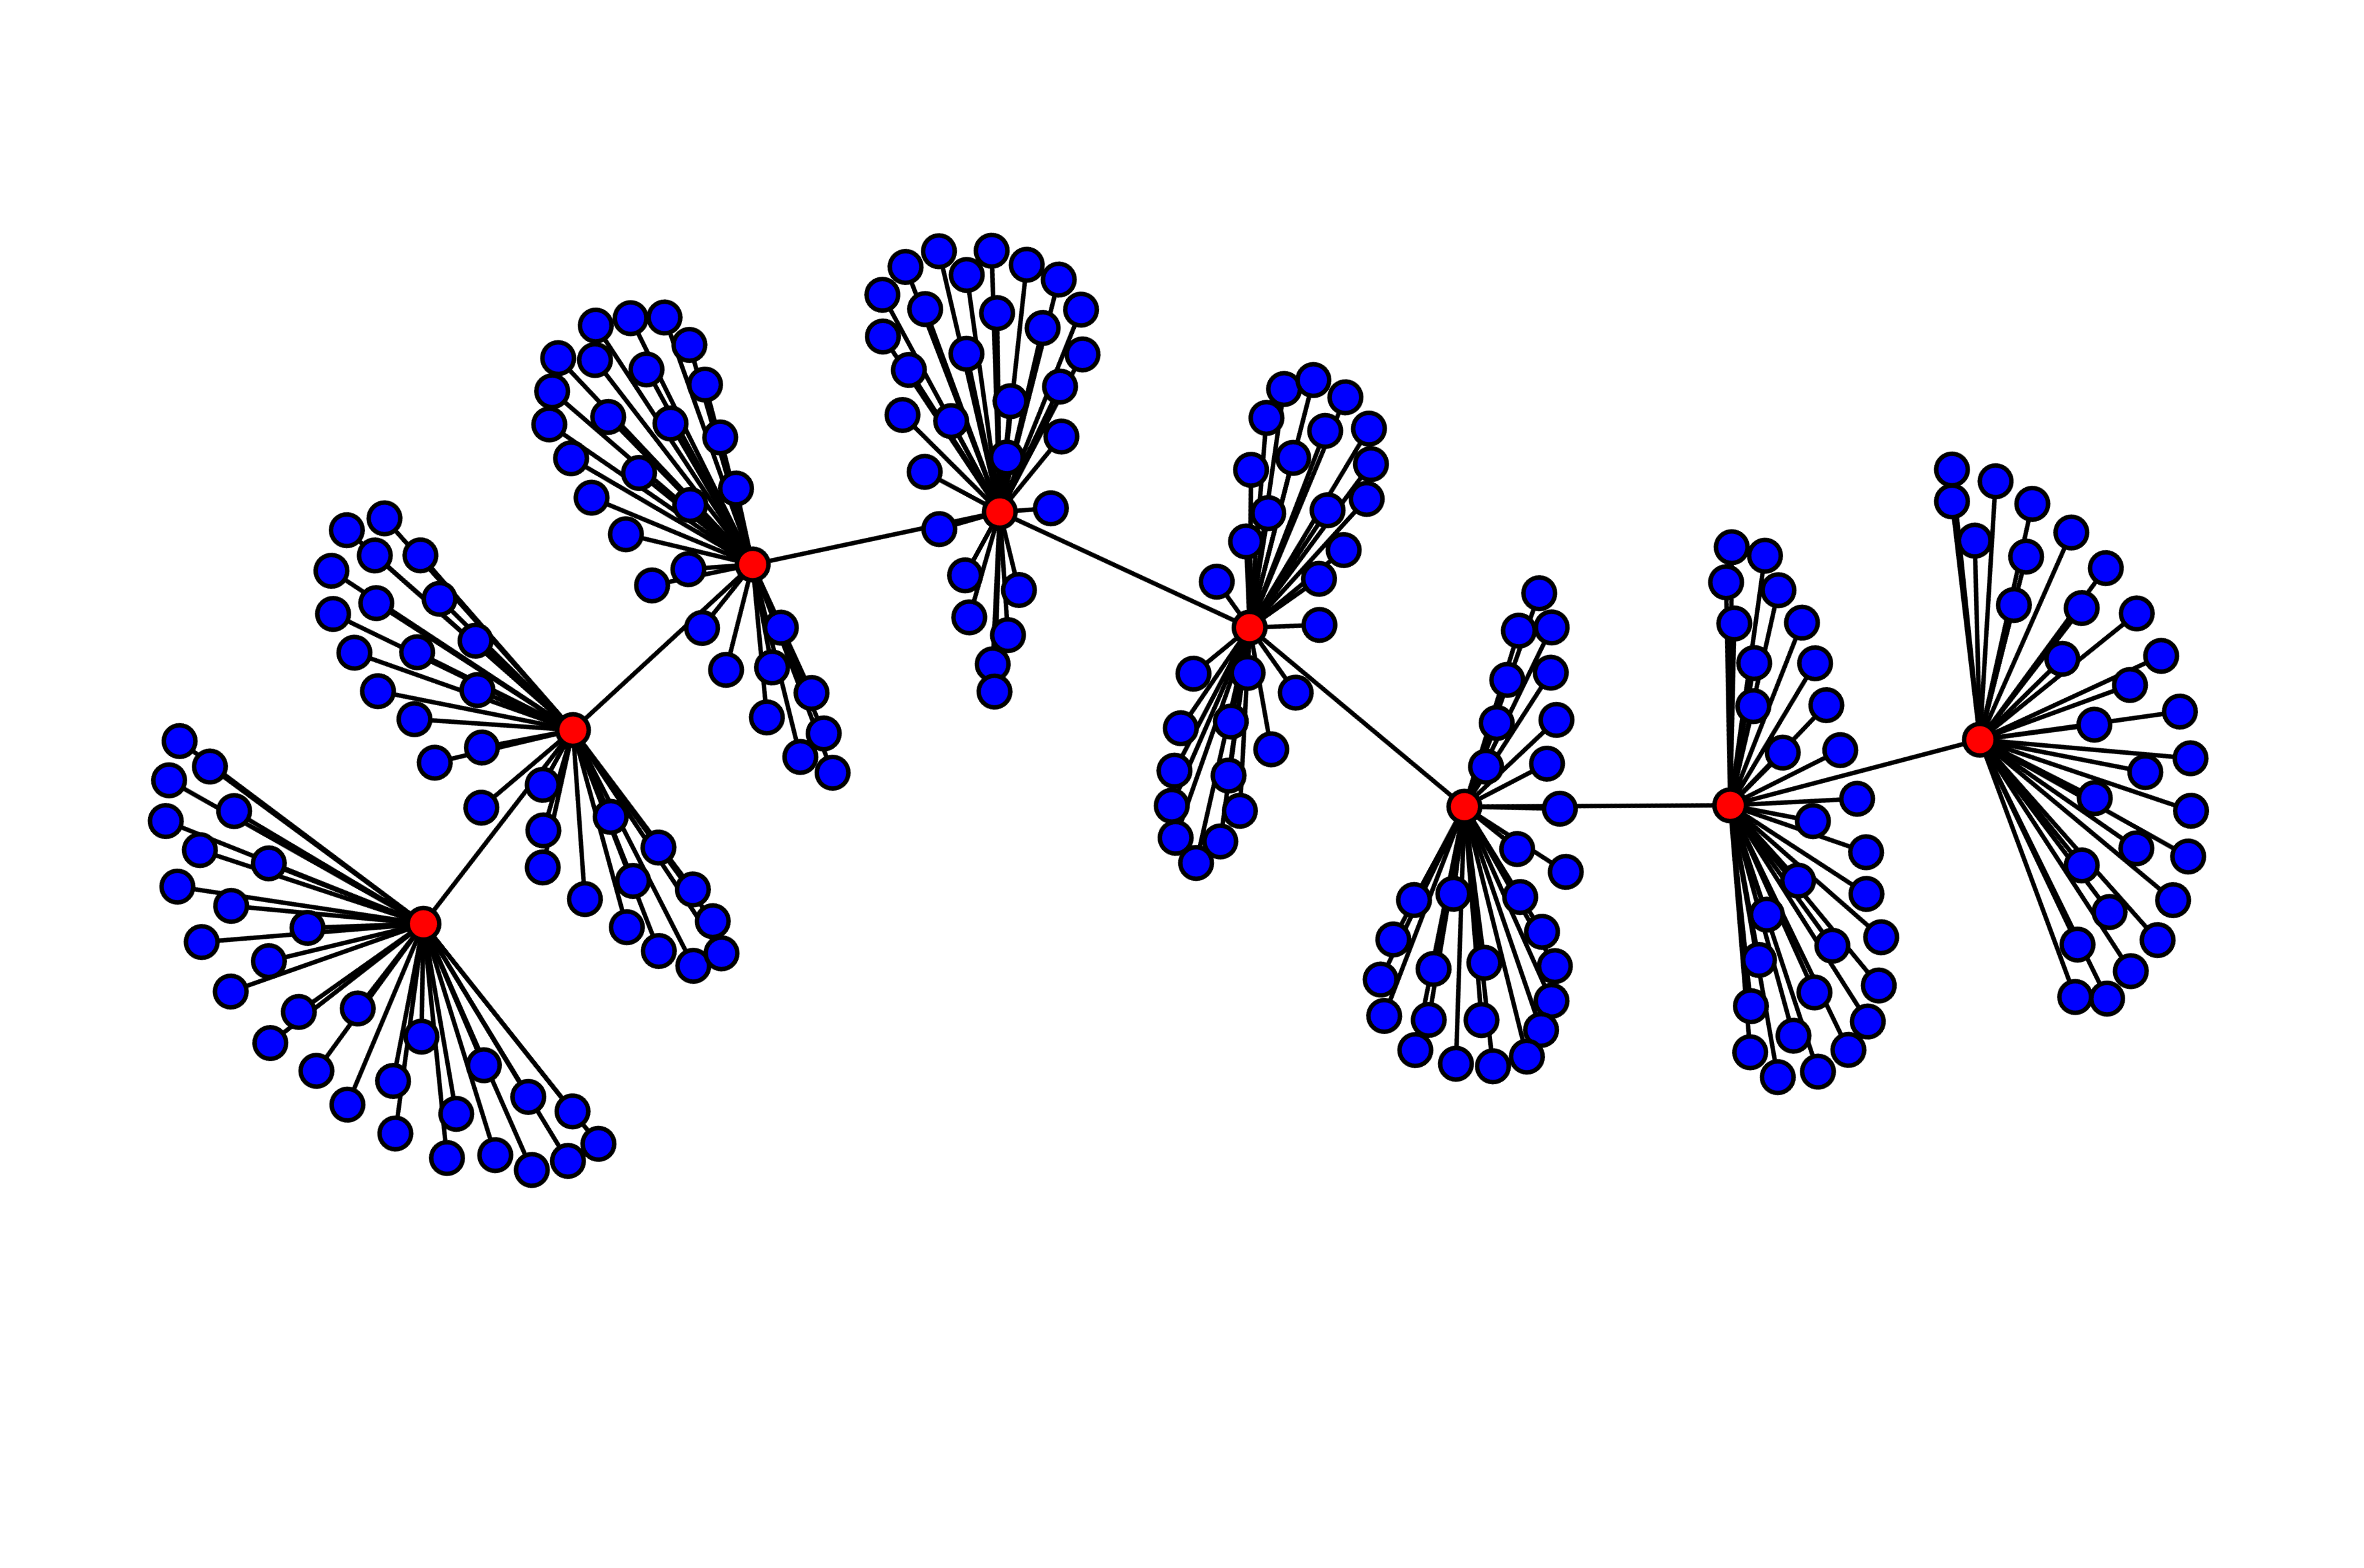
\includegraphics[width=\textwidth]{img/full-graph}
    \caption{Grafo representando uma rede com 248 entidades}
    \label{fig:full-graph}
\end{figure}

Atualizações na topologia como, remover e adicionar entidades na rede, foram
executados.
A visualização da rede atualiza junto com as alterações no grafo.

\section{Identificação de tráfego}

\section{Rede Nacional de Pesquisa (RNP-IPÊ)}
